\documentclass[sigconf]{acmart}


\usepackage{xcolor}

\usepackage{float}
\usepackage{siunitx}


\newif\iffinal

% \finaltrue

\iffinal
  \newcommand{\tyler}[1]{}
  \newcommand{\ian}[1]{}
  \newcommand{\kyle}[1]{}
\else
  \newcommand{\tyler}[1]{{\textcolor{cyan}{ tyler: #1 }}}
  \newcommand{\ian}[1]{{\textcolor{red}{ Ian: #1 }}}
  \newcommand{\kyle}[1]{{\textcolor{purple}{ Kyle: #1 }}}
\fi


%%
%% \BibTeX command to typeset BibTeX logo in the docs
\AtBeginDocument{%
  \providecommand\BibTeX{{%
    \normalfont B\kern-0.5em{\scshape i\kern-0.25em b}\kern-0.8em\TeX}}}


\newcommand{\name}{Xtract}
\newcommand{\funcx}{$f$\kern-0.18em\emph{unc}\kern-0.05em X}

\acmConference{Fifth International Workshop on Serverless Computing (WoSC)}{2019}{Davis, CA}

\begin{document}


\title{Harnessing Serverless to Extract File Metadata at the Edge}


\author{Tyler J. Skluzacek} 
\affiliation{University of Chicago}
\email{skluzacek@uchicago.edu}



\renewcommand{\shortauthors}{Skluzacek et al.}

\begin{abstract}
\tyler{max 100 words}

\tyler{GRAND-er. be more dramatic. }
\kyle{Maybe here you could say. Lots of data. Its created and stored in different places. 
We need to rethink the siloed and antiquated file system approach and instead think
of data in one global index of metadata (i.e., a data ocean -- just made up this term, not sure
if I like it). To do this we need to be able extract metadata
from where data exists. We propose a fluid, serverless middleware in which extractors
are dynamically determined and executed wherever it makes most
sense (e.g., at the edge, cloud, computing center, ...)}

The rapid increase in the number of data sources and sizes will prove largely 
useless if these data are not findable, interpretable, or reusable. In this work 
we propose a middleware architecture called Xtract that leverages serverless 
computing to simultaneously extract metadata across a continuum of heterogeneous edge 
devices, from IoT to HPC to 
laptops. Xtract will enable the curation of an atomic multi-site data lake in which the
resources can make intelligently scale and move data in order to optimize for various 
SLAs.


\end{abstract}

\begin{CCSXML}
<ccs2012>
<concept>
<concept_id>10002951.10003227.10010926</concept_id>
<concept_desc>Information systems~Computing platforms</concept_desc>
<concept_significance>500</concept_significance>
</concept>
<concept>
<concept_id>10002951.10003317.10003365.10003366</concept_id>
<concept_desc>Information systems~Search engine indexing</concept_desc>
<concept_significance>300</concept_significance>
</concept>
<concept>
<concept_id>10002951.10003317.10003318.10003319</concept_id>
<concept_desc>Information systems~Document structure</concept_desc>
<concept_significance>100</concept_significance>
</concept>
<concept>
<concept_id>10010405.10010497.10010500.10010503</concept_id>
<concept_desc>Applied computing~Document metadata</concept_desc>
<concept_significance>500</concept_significance>
</concept>
</ccs2012>
\end{CCSXML}

\ccsdesc[500]{Information systems~Computing platforms}
\ccsdesc[500]{Applied computing~Document metadata}
\ccsdesc[300]{Information systems~Search engine indexing}
\ccsdesc[100]{Information systems~Document structure}

\keywords{data lakes, serverless, metadata extraction, file systems, materials science}

\maketitle


\section{Introduction}

%As IoT, scientific instruments, and personal computing devices generate large quantities of streaming data, 
%running compute tasks on predefined resource allocations proves generally ineffective. For one, a given 
%allocation may not be available---for instance, a shorter-duration task might spend an inordinate amount of time in an 
%HPC task queue. Additionally for some workloads, moving data to dedicated clusters can be prohibitively expensive, 
%and 

% For instance, electron 
% microscopy studies must first determine an image's quality before processing it, making every low-quality image transferred 
% a sunk cost. 
\kyle{this is similar to workshop paper. what are the rules on re-using text?}
Advances in scientific instruments, computational capabilities, and the proliferation of IoT devices
have increased the volume, velocity, and variety of data. 
As a result, organizations are increasingly adopting data-driven enterprise and research practices, 
in which data are collected, stored for long periods of time, shared, 
and reused.
Unfortunately, these factors create new data management challenges, 
not least of which is the need for data to be adequately described
for it to be generally useful. Without descriptive metadata, data
may become unidentifiable, siloed, and in general, 
not useful to either one's own organization or the broader open-source community. 
Unfortunately, organizing and annotating data is a time-consuming process
and the gulf between data generation rates
and the finite management capabilities of researchers
continues to grow. To increase the value and usefulness of scientific data, 
new methods are required to automate the extraction and association 
of rich metadata that describe not only the data themselves, but
also their structure and format, provenance, and administrative information.

%Data lakes have become a popular paradigm for managing large and 
%heterogeneous data from various sources. 
%A data lake contains a collection of data in different formats, 
%accompanied by metadata describing those data. 
%Unfortunately, the data deluge and the desire to store all data
%for eternity can quickly turn a data lake into a ``data 
%swamp''~\cite{skluzacek2018skluma}---a term used to describe the situation in which the data 
%stored in the data lake lack the metadata necessary to be 
%discoverable, understandable, and usable. Without automated and scalable 
%approaches to derive metadata from scientific data, the utility of 
%these data are reduced. This problem is 
%especially prevalent in science as 
%datasets can be enormous (many petabytes),
%are created and shared by dynamic collaborations, 
%are often collected under tight time constraints where data management processes become afterthoughts, 
%and for which preservation is important for purposes of reproducibility and reuse. 

\tyler{Add note here about the edge}
Extracting metadata from enterprise and scientific data is a complex task. 
Data repositories may exceed millions of files and petabytes of data;
data are created at different rates, by different people; 
and there are an enormous number of data formats and conventions. 
Some~\cite{egan2003vizier, welter2013nhgri, irods, dataverse} have created 
systems to manage metadata catalogs that
support the organization and discovery of research data. However, these approaches typically 
require that users provide metadata and that curators continue to organize data over time.
While metadata can be rapidly extracted from some data types, others, such as
images and large hierarchical file formats can require the use of multiple extraction methods.  
As a result, the metadata extraction process must be scalable to process large numbers
of files, flexible to support different extraction methods, and extensible
to be applied to various scientific data types and formats.

Serverless computing, and in particular function as a service (FaaS),
provides an ideal model for managing the execution of
many short-running extractors on an arbitrarily large number of files. 
Serverless computing abstracts computing resources from the user, enabling
the deployment of applications without consideration for the physical and virtual infrastructure on which 
they are hosted.FaaS allows users to register programming functions with predefined input signatures. 
Registered functions can subsequently be invoked many times
without the need to provision or scale any infrastructure.

\tyler{need to mention the name of our system first} \kyle{Do other papers have a separate RW section?}
We are not the first to construct an architecture to automatically extract metadata from repositories. 
For example, ScienceSearch~\cite{rodrigo2018sciencesearch} uses 
machine learning techniques to extract metadata from a dataset served by the National Center for Electron Microscopy (NCEM). 
Most of data in this use case are micrograph images, but additional contextual metadata are derived from file system 
data and free text proposals and publications. Like \name{}, ScienceSearch 
provides a means for users to extensibly switch metadata extractors to suit a given dataset.  
Brown Dog~\cite{padhy2015brown} is an extensible metadata extraction platform, 
providing metadata extraction services for a number of 
disciplines ranging from materials science to social science.
Unlike \name{}, Brown Dog requires that files are uploaded for extraction. 

In this paper we propose the use of FaaS for mapping the metadata extraction problem to a 
collection of granular metadata extractor functions. 
We describe how such a model can support the flexibility, scalability, and extensibility required
for scientific metadata extraction. 
Rather than rely on commercial FaaS systems, we use a distributed FaaS model 
that overcomes the limitation of moving large amounts of data to the cloud. 
Instead, we are able to push
metadata extractors to the edge systems on which the scientific data reside. 

Our prototype system, \name{}, provides high-throughput and on-demand metadata 
extraction that enables the automated creation of rich, searchable data lakes from previously unsearchable data swamps. 
\name{} uses the \funcx{} serverless supercomputing platform~\cite{chard2019serverless}
to execute functions across diverse and distributed computing infrastructure.
The contributions of \name{} are the following: 



The primary goal of this work is the following: 

\begin{itemize}
\item Implement and evaluate a serverless metadata extraction system
\item Enable users to deploy endpoints and invoke metadata extraction functions on the edge
\item Create comprehensive, searchable indexes of files across multiple devices
\item Explore intelligent self-optimization methods subject to a number of constraints, including compute time, 
current allocation availability, monetary cost, and security requirements (e.g., HIPAA).
\end{itemize}


\section{Approach}
\label{sec:approach}

\name{} is implemented as a service via which users can submit
requests to extract metadata from a collection of files.
\name{} first crawls the specified files and determines
an initial set of extractors to apply to them. 
As outlined above, the extractors may be executed
either centrally on the \name{} server or remotely alongside
the data. As processing continues, \name{} assembles 
a metadata document for each file and dynamically selects
other extractors to apply.

%\ryan{Explain here that we have the ability to do edge but our prototype leverages petrelkube -- which is an edge device for all 
%intents and purposes as we still fire jobs into funcx}

%\name{} is implemented as a RESTful web service and is 
\name{} is deployed on Amazon Web Services (AWS) and makes use
of various services. The main \name{} service
is deployed on an AWS Elastic Compute Cloud instance.
\name{} manages state in an AWS Relational Database Service (RDS)
instance. Each extraction request is stored in the database
and the state is updated throughout the extraction process. 
\name{} is able to send the derived metadata to an external
metadata catalog such as a Globus Search index.
The \name{} architecture is shown in Figure~\ref{fig:arch}.

\begin{figure}[t]
	\centering
	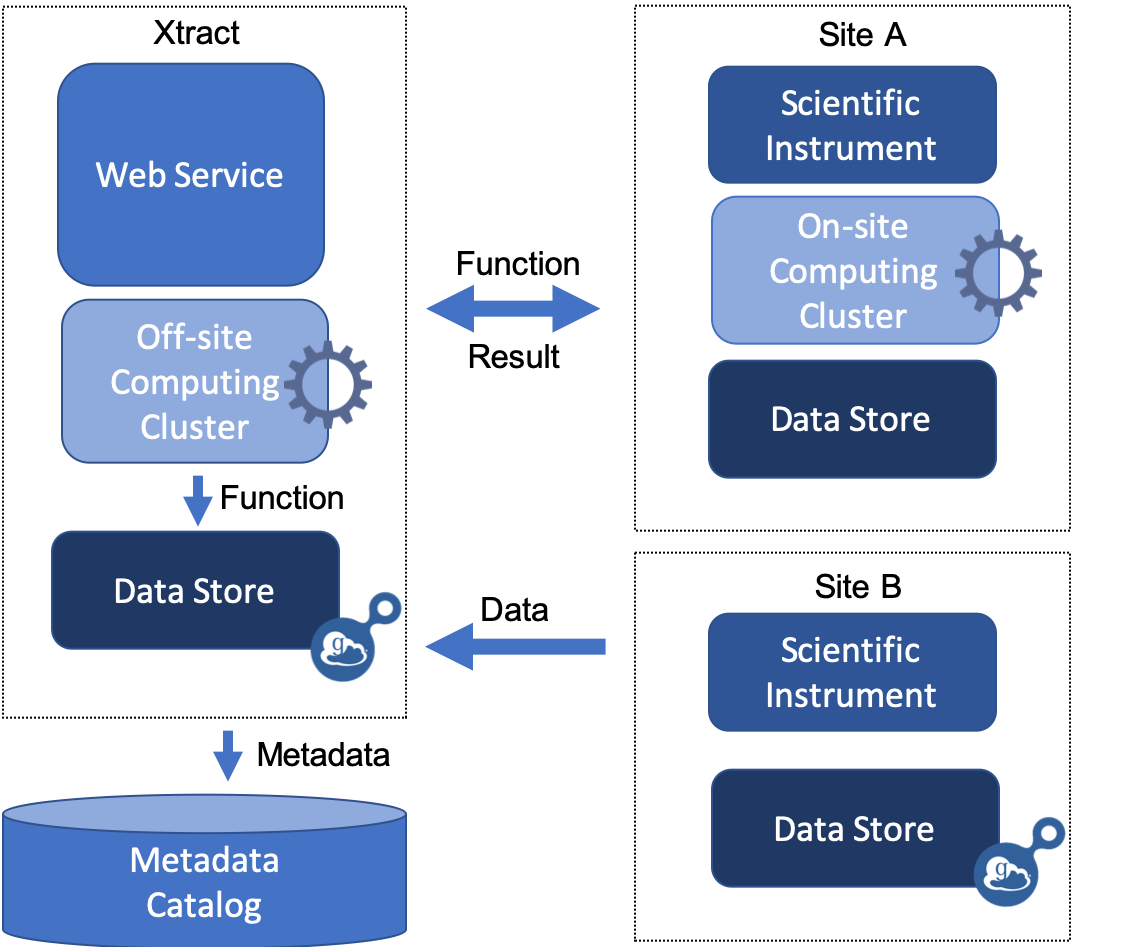
\includegraphics[scale=0.3]{figs/new-arch.png}
	\caption{Overview of the \name{} architecture. For \textit{Site A} functions are transmitted to the remote resource and performed on local computing resources, returning metadata to the \name{} service. \textit{Site B} lacks suitable local
	computing capabilities, requiring data to be staged to \name{} for analysis.}
	\label{fig:arch}
\end{figure}

\subsubsection{Metadata Extractors}
\name{} is designed to execute its extractors centrally or on edge storage systems near to where
data are stored. 
Our implementation uses the \funcx~\cite{chard2019serverless} FaaS platform 
to deploy and run extractors. 
\funcx{} is specifically designed to integrate with research computing 
cyberinfrastructure and enable a FaaS execution interface. 
\funcx{} builds upon the Parsl~\cite{babuji2019parsl} parallel programming library to 
manage the execution of functions in containers on arbitrary compute resources. 
\funcx{} enables \name{} to execute metadata extraction functions at any registered 
and accessible \funcx{} endpoint. 
We deploy the prototype with a co-located endpoint for central extraction
and use remotely deployed endpoints for edge extraction.

Each \name{} metadata extractor and its dependencies are wrapped in a Docker container
such that it can be executed in different locations. 
We have published each extractor container to \funcx{} and registered a \funcx{} function for 
each extractor. The function is responsible for invoking the extractor and returning the 
resulting metadata as a JSON dictionary. 

\funcx{} enables \name{} to reliably scale to thousands of nodes and deploy 
metadata extraction tasks on arbitrary computing resources. 
\name{} can make use of any accessible \funcx{} endpoint to process data at the edge, 
sending extractor codes and containers to the \funcx{} endpoint for execution. In addition, 
\funcx{} supports Singularity and Shifter, allowing \name{} extractors to be executed
on various high performance computing systems. 

\name{} implements a comprehensive security model using Globus Auth~\cite{tuecke2016globus}. 
All interactions with the \name{} Web service are secured with Globus Auth. 
Users can authenticate with \name{} using one of 
several hundred identity providers, including many institutions. 
\name{} uses Globus Auth OAuth~2 flows to stage data on behalf
of authenticated users. \name{} first verifies a user identity, requests an access
token to perform data transfers on their behalf, and then uses Globus to stage
data from remote storage to the \name{} extractor. 
Finally, the resulting metadata are published into the search index using a Globus Search
access token. The search index is configured with a \textit{visible\_to} field, restricting
discovery to authenticated users.


\section{Evaluation Plan}
\label{sec:eval}

We intend to index real science use cases, particularly those in which individual data files are heterogeneous 
or geographically distributed. For each, we intend to explore how to optimize the system across dimensions of 
total compute time (SLAs), monetary cost, security requirements, and resource availability.

We target the following real-world data sets: 

We have already generated an index of the Carbon Dioxide Information Analysis Center (CDIAC), a collected dataset of 
emissions data containing over 500,000 files (330+ GB) and 10,000 unique file extensions. The archive contains little 
descriptive metadata and includes a number of irrelevant files, such as debug-cycle error logs and Windows Desktop 
shortcuts.  We deployed this metadata extraction service in the cloud and moving the data to the cloud, but we expect 
to see significant time and monetary savings by moving the data to the cloud.  

The Materials Data Facility~\cite{blaiszik2016materials, blaiszik2019mdf}
is a centralized hub for publishing, sharing, and discovering materials science data. 
The MDF stores many terabytes of data from many different research groups, covering many disciplines of 
materials science, and with a diverse range of file types.
The downside of the expansive range of materials data held by the MDF 
is that it can be difficult for users to find data relevant to their science.
The MDF reduces the ``data discovery" challenge by hosting a search index that provides access to metadata from the 
files (e.g., which material was simulated in a certain calculation).
The data published by the MDF is primarily stored on storage at the National Center for Supercomputing Applications
(NCSA) and is accessible via Globus.  

Petrel? Running out of room. 

Globus~\cite{ananthakrishnan2018globus} manages petabytes of files over tens of thousands of individual user endpoints between research labs, 
universities, industry, and home computing devices. Many \tyler{???} users elect to have all or part of their data publicly 
shared with the rest of the Globus community. \kyle{private sharing could also be indexed} Xtract lends itself well to Globus as Globus already deploys an 
endpoint on the compute node.  We intend to deploy the funcX endpoint as part of the Globus endpoint software, and 
execute secure metadata extraction over all available petabytes. Globus is particularly useful in studying multi-site 
metadata extraction, as users generally have multiple active endpoints. \tyler{more detail}. 



\section{Conclusion}
\label{sec:conc}

Metadata extraction at the edge will make previously siloed data searchable and usable by researchers, 
industries with cumbersome data scales, and individuals simply wanting a centralized index across 
each of their files. 


\begin{acks}

This research is conducted under the guidance of Dr. Ian Foster and Dr. Kyle Chard of the 
University of Chicago and Argonne National Lab. This work is made possible in part by the contributions
of Ryan Chard, Yadu N. Babuji, Zhuozhao Li, and Ryan Wong. 


\end{acks}
\bibliographystyle{ACM-Reference-Format}
\bibliography{wosc}


\end{document}
\endinput
